% ****************************************************************************************************
% Chapter 4: Feature Engineering and Clinical Scores
% ****************************************************************************************************

\chapter{Feature Engineering and Clinical Scores}
\label{ch:features}

The heart of any applied machine learning project is not the model. It is the features. A carefully chosen feature can make a weak model strong; a poorly chosen one can make the best architecture useless. In medical machine learning, the feature set also serves a second purpose: it is the primary vocabulary through which the model makes contact with clinical practice. If my features align with how nurses and physicians actually think about acuity, the model has a chance of learning something generalisable. If my features are arbitrary projections of arbitrary columns, it does not.

This chapter describes the 65 tabular features used in my best pipeline, along with the 50 text embedding components derived from the chief complaint (I treat the text separately in Chapter~\ref{ch:embeddings}). Together they form a 115-dimensional input vector per patient. I explain how each category of features was constructed, why it was chosen, and in several cases, which alternatives I tried and abandoned.

\section{The Guiding Principles}

Before I list the features, it is worth stating the three principles that guided their construction.

\paragraph{No leakage.} Every feature must be computable at the moment of triage, using only information available at that moment. Medication records from during the hospital stay cannot be used, because they do not exist at triage time. The number of prior ED visits must count strictly earlier visits, not the current one. The chief complaint text is available; the diagnosis written three hours later by an ED physician is not. This is the principle I discussed in Chapter~\ref{ch:mimic}. I return to it repeatedly below because it is easy to violate without noticing.

\paragraph{Clinical grounding.} Wherever possible, I reach for features with established clinical meaning. A composite score like NEWS2 \citep{rcp2017news2}, used in practice by hospitals across the United Kingdom and Ireland, brings a readable clinical interpretation that a generic polynomial feature cannot. When I use derived features like shock index or mean arterial pressure, these are derived quantities that appear in textbooks, not products of automated feature search.

\paragraph{Honest ablation.} Features were added when they helped, and removed when they did not. Several features I initially expected to be useful, the Rapid Emergency Medicine Score, individual vital-sign abnormality flags, age-decile vital z-scores, ended up contributing nothing or next to nothing, and were dropped. I document these dead ends alongside the successes.

\begin{remarkbox}[Why Only 65 Features?]
One might expect that more features would generally be better. They are not. Gradient-boosted decision trees, my chosen family of models, handle irrelevant features gracefully but not costlessly. Each irrelevant feature increases the search space during training, increases the risk of overfitting on small folds, and dilutes the importance scores I rely on for explainability. I settled on 65 tabular features through iterative pruning: features with near-zero importance across folds were removed, and the final set is the smallest one that does not sacrifice performance. This is the opposite of the ``feed every column into XGBoost'' style that sometimes wins Kaggle leaderboards. It is also the style that more closely resembles how a clinician would reason.
\end{remarkbox}

\section{Raw Vital Signs}

The six vital signs measured at triage form the backbone of my feature set. These are the same vital signs a nurse would measure at any ED in the world, and they are the first features any sensible clinical prediction system would use.

\begin{itemize}
 \item \texttt{temperature}, body temperature in degrees Celsius.
 \item \texttt{heartrate}, heart rate in beats per minute.
 \item \texttt{resprate}, respiratory rate in breaths per minute.
 \item \texttt{o2sat}, peripheral oxygen saturation (SpO$_2$), a percentage.
 \item \texttt{sbp}, systolic blood pressure in mmHg.
 \item \texttt{dbp}, diastolic blood pressure in mmHg.
\end{itemize}

Each of these is a single numeric value per visit, extracted directly from the \texttt{triage} table with minimal cleaning. Ranges are biologically constrained, a human heart rate below 30 or above 240 is almost certainly a measurement error, but I did not apply aggressive clipping. LightGBM handles outliers gracefully through its tree-based splits, and overly strict clipping can remove genuine physiological extremes (a patient in cardiac arrest may have a heart rate well outside the ``normal'' range).

The diagnostic value of raw vitals is considerable. A systolic blood pressure below 90 mmHg or an oxygen saturation below 92\% immediately raises the acuity level in every standard triage system \citep{rcp2017news2}. But raw vitals are also noisy, a single measurement at triage captures one moment of a fluctuating physiological state, and they are not sufficient on their own. They become most informative when combined.

\section{Engineered Vital Signs}

From the six raw vitals, I derive eight further numeric features. These derivations are all standard in clinical practice and serve to make latent relationships explicit to the model.

\subsection*{Shock Index}

The shock index is the ratio of heart rate to systolic blood pressure:
\[
\text{shock\_index} = \frac{\text{heart rate}}{\text{systolic BP}}
\]

A shock index above 0.9 is associated with haemodynamic instability even when heart rate and blood pressure appear individually normal. This is a classic example of a feature that encodes clinical reasoning the model could not easily learn from the raw inputs alone: a patient with heart rate 110 and SBP 110 has a shock index of 1.0, which suggests compensated shock, but neither raw value in isolation would trigger an alarm. The shock index makes this explicit.

\subsection*{Pulse Pressure and Mean Arterial Pressure}

From systolic and diastolic blood pressure, I derive two further quantities:
\begin{align*}
\text{pulse\_pressure} &= \text{SBP} - \text{DBP} \\
\text{MAP} &= \frac{\text{SBP} + 2 \times \text{DBP}}{3}
\end{align*}

Pulse pressure reflects the compliance of the aorta and large arteries; mean arterial pressure is a weighted average representing the average pressure perfusing the organs across the cardiac cycle. Both are standard in cardiovascular assessment. The weighting in MAP reflects the fact that the heart spends more of its cycle in diastole than in systole.

\subsection*{Pain Score}

The \texttt{pain} column in MIMIC-IV-ED is free text rather than a clean numeric field. A triage nurse may enter \texttt{7}, \texttt{7/10}, \texttt{moderate}, \texttt{none}, \texttt{unable to assess}, or any of a dozen other strings. I parsed this to a numeric feature \texttt{pain\_numeric} using a regex that extracts the first number and clips to $[0, 10]$. Non-numeric entries became missing values. The preprocessing looks like this:

\begin{lstlisting}[language=Python, caption={Pain score parsing. The regex handles formats like ``7'', ``7/10'', and ``pain 8''. Values outside the 0--10 scale, including text-only entries, become missing.}]
def parse_pain(val):
 if pd.isna(val):
 return np.nan
 m = re.search(r"\b(\d+(?:\.\d+)?)\b", str(val).strip().lower())
 if m:
 v = float(m.group(1))
 return v if v <= 10 else np.nan
 return np.nan

df["pain_numeric"] = df["pain"].apply(parse_pain)
\end{lstlisting}

\subsection*{Clinical Composite Scores: NEWS2 and qSOFA}

The remaining four engineered vitals are composite scores. These are the most clinically meaningful features I add, and they deserve detailed explanation.

\paragraph{NEWS2.} The National Early Warning Score 2, published by the Royal College of Physicians in 2017 \citep{rcp2017news2}, is a bedside risk-stratification tool used across the UK NHS and in many hospitals internationally. It aggregates seven physiological parameters into a single integer score from 0 to 20. Higher scores indicate greater risk of clinical deterioration, and specific thresholds trigger escalation protocols: a score of 5 or more prompts urgent clinical review, and a score of 7 or more prompts emergency review.

My implementation uses five of the seven NEWS2 components, listed in Table~\ref{tab:news2-scoring}. The two components I omit are supplemental oxygen (a binary indicator of whether the patient is on $O_2$ support) and level of consciousness (the AVPU scale: Alert / Voice / Pain / Unresponsive). Neither is recorded in the MIMIC-IV-ED triage table. This is a limitation of the data source, not of my methodology; if these fields were available, incorporating them would be mechanical.

\begin{table}[htbp]
 \centering
 \caption[NEWS2 scoring table as implemented]{The partial NEWS2 scoring table used in this work. Five of the seven standard components are included; supplemental oxygen and AVPU consciousness level are unavailable in MIMIC-IV-ED triage data. My maximum score is $5 \times 3 = 15$, versus $15$ (base) $+ 2$ (O$_2$) $+ 3$ (AVPU) $= 20$ for full NEWS2. The SpO$_2$ thresholds follow Scale 1 (for patients not on supplemental O$_2$).}
 \label{tab:news2-scoring}
 \small
 \begin{tabular}{lcccccc}
 \toprule
 Parameter & \multicolumn{5}{c}{Score contribution} \\
 \cmidrule(lr){2-6}
 & 3 & 2 & 1 & 0 & 1 \\
 \midrule
 Respiratory rate (per min) & $\leq 8$ &, & 9--11 & 12--20 & 21--24* \\
 SpO$_2$ (\%) & $\leq 91$ & 92--93 & 94--95 & $\geq 96$ &, \\
 Systolic BP (mmHg) & $\leq 90$ & 91--100 & 101--110 & 111--219 & $\geq 220$** \\
 Heart rate (per min) & $\leq 40$ &, & 41--50 & 51--90 & 91--110 \\
 Temperature (°C) & $\leq 35.0$ &, & 35.1--36.0, 38.1--39.0 & 36.1--38.0 &, \\
 \bottomrule
 \end{tabular}
 \begin{flushleft}\small
 *Respiratory rate $\geq 25$ scores 3. **SBP $\geq 220$ scores 3. Temperature $\geq 39.1$ scores 2. Table condensed for readability.
 \end{flushleft}
\end{table}

The score is computed as the integer sum of the five component contributions, with NaN propagation for any missing vital. Downstream, missing composite scores are imputed using the median within each training fold.

\paragraph{qSOFA.} The quick Sequential Organ Failure Assessment score \citep{singer2016sepsis3} was introduced in 2016 as a bedside tool for identifying patients at risk of sepsis-related deterioration. It has three components, each scoring 0 or 1:

\begin{enumerate}
 \item Respiratory rate $\geq 22$ per minute.
 \item Systolic blood pressure $\leq 100$ mmHg.
 \item Altered mental status (GCS $< 15$, or clinically equivalent).
\end{enumerate}

My implementation uses two of the three components. The altered mental status criterion requires a Glasgow Coma Scale assessment, which is not recorded in MIMIC-IV-ED's triage table. My partial qSOFA therefore ranges from 0 to 2 rather than the standard 0 to 3. A qSOFA score of 2 or more (in the full three-component version) is associated with a substantially increased risk of in-hospital mortality in suspected sepsis \citep{seymour2016qsofa}.

\paragraph{Age-Adjusted Shock Index.} The shock index above does not account for age. Elderly patients often have baseline cardiovascular compensation that keeps their heart rate low and blood pressure normal even in early shock, a phenomenon sometimes called compensated shock in the elderly, distinct from the compensated shock in young patients I discuss in Chapter~\ref{ch:fairness}. I compute an age-adjusted shock index:
\[
\text{age\_shock\_index} = \text{shock\_index} \times \text{age}
\]
The product scales shock index by age directly, amplifying the signal for elderly patients whose compensated physiology may mask deterioration. The feature was important in my model: it appeared in the top 10 by LightGBM gain importance in several experimental runs.

\paragraph{Age-Stratified Vital Abnormality Count.} My fourth composite, \texttt{n\_abnormal\_vitals}, counts the number of vital signs that fall outside age-adjusted normal ranges. The thresholds are listed in Table~\ref{tab:age-strat-thresholds}, with separate bounds for elderly ($\text{age} \geq 70$) and non-elderly patients. Nine individual binary flags are summed, producing a score from 0 to 9.

\begin{table}[htbp]
 \centering
 \caption[Age-stratified vital abnormality thresholds]{Thresholds used to define abnormal vital signs, stratified by age. The count of how many thresholds are crossed forms the \texttt{n\_abnormal\_vitals} composite feature.}
 \label{tab:age-strat-thresholds}
 \small
 \begin{tabular}{lcc}
 \toprule
 Threshold & Non-elderly ($<$ 70) & Elderly ($\geq$ 70) \\
 \midrule
 Heart rate high & $> 100$ & $> 90$ \\
 Heart rate low & $< 50$ & $< 50$ \\
 Systolic BP low & $< 90$ & $< 100$ \\
 Systolic BP high & $\geq 180$ & $\geq 180$ \\
 SpO$_2$ low & $< 94\%$ & $< 92\%$ \\
 Temperature high & $> 38.5$°C & $> 38.0$°C \\
 Temperature low & $< 35.5$°C & $< 35.5$°C \\
 Respiratory rate high & $> 22$ & $> 20$ \\
 Respiratory rate low & $< 10$ & $< 10$ \\
 \bottomrule
 \end{tabular}
\end{table}

\begin{notebox}[Why Stratify by Age at All?]
The rationale is that physiological ``normal'' ranges are themselves age-dependent. An 80-year-old patient with a heart rate of 95 is likely showing early stress; the same heart rate in a 25-year-old is within normal range and not alarming. Encoding this as binary flags lets the model learn age-dependent thresholds without having to discover them from the raw data. I chose 70 as the stratification boundary as a compromise between the 65-year threshold often used in clinical guidelines and the 75-year threshold used in some geriatric medicine literature. The exact boundary was not heavily optimised, a reader interested in precision medicine could reasonably use finer age decile z-scores, which I tried in a separate experiment (Chapter~\ref{ch:fairness}) with mixed results.
\end{notebox}

\section{Missingness as Signal}

Six additional features record whether each vital sign was missing at triage: \texttt{temperature\_missing}, \texttt{heartrate\_missing}, and so on.

In a typical tabular ML problem, missingness is nuisance: you impute the missing values and move on. In clinical data, missingness is information. A vital sign is missing because a nurse did not take it, which is not a random event. In practice, missing vitals in the triage table correlate systematically with acuity: critically ill patients arriving by ambulance may be moved directly to a resuscitation bay without a complete triage workup, while walk-in patients with minor complaints routinely have every vital measured. Temperature in particular is frequently missing in ESI-1 cases where immediate stabilisation takes priority.

Including explicit missingness flags lets the model learn this signal without conflating it with imputed values. After flag extraction, actual missing numeric values are filled with the training-fold median in each cross-validation split. The median is a reasonable choice for continuous physiological variables with heavy tails and is less sensitive to outliers than the mean.

\section{Demographics and Arrival Mode}

Seven features describe the patient and how they arrived.

Four are categorical: \texttt{gender}, \texttt{race}, \texttt{age\_group} (categorical age bucket), \texttt{insurance}, \texttt{language}, and \texttt{marital\_status}. Gradient-boosted tree models handle these natively through LightGBM's categorical feature support, which uses a specialised split-finding algorithm that partitions categorical values rather than one-hot encoding them. I included these features despite some misgivings, insurance and language in particular raised fairness concerns that became important in Chapter~\ref{ch:explainability} when SHAP analysis revealed them as top-ranked features, but chose to retain them and audit their effects downstream.

Age itself is recorded numerically as \texttt{age}, computed from MIMIC's de-identified \texttt{anchor\_age} field plus the offset from the anchor year. The computation is:
\begin{lstlisting}[language=Python]
df["age"] = (df["anchor_age"]
 + (df["intime"].dt.year - df["anchor_year"])).clip(0, 120)
\end{lstlisting}

The cyclic encoding of arrival hour deserves explanation. I do not use the raw hour of day (0 to 23) because that encoding misleadingly places 23:00 and 00:00 far apart in feature space when clinically they are adjacent. Instead, I decompose the hour into two features:
\begin{align*}
\text{arrival\_hour\_sin} &= \sin\!\left(\frac{2\pi h}{24}\right) \\
\text{arrival\_hour\_cos} &= \cos\!\left(\frac{2\pi h}{24}\right)
\end{align*}
where $h$ is the hour. This preserves cyclic structure: midnight and 1 AM are close in both components, as are 11 PM and midnight. The model can learn that arrivals in the early hours of the morning have different characteristics from afternoon arrivals, a real effect in ED data, where overnight arrivals tend to be higher acuity because patients with minor complaints are less likely to seek care at 3 AM.

The \texttt{arrival\_transport} categorical feature records how the patient arrived: ambulance, helicopter, walk-in, or transfer from another facility. Ambulance arrival in particular is a strong predictor of higher acuity and is consistently among the top 10 features in my LightGBM importance rankings.

\section{Medications and Comorbidities}

Twenty-nine features encode the patient's medical history. These split into two groups: current medications (from the \texttt{medrecon} table) and prior diagnoses (from the \texttt{diagnoses\_icd} table).

\subsection*{Pre-Admission Medications}

The \texttt{medrecon} table is, by MIMIC design, a record of the patient's home medications, the drugs they were taking before coming to the ED. It is populated during the medication reconciliation process that happens at triage or shortly after, where a nurse asks the patient (or reviews their pharmacy record) about current medications. This is distinct from \texttt{pyxis}, which records medications dispensed during the hospital stay and which I do not use because it would represent leakage.

Every medication in \texttt{medrecon} carries an Enhanced Therapeutic Classification (ETC) description, a drug ontology that groups medications into therapeutic classes. I use these descriptions to assign each medication to one of 13 clinically meaningful classes through case-insensitive substring matching. Table~\ref{tab:med-classes} lists the classes.

\begin{table}[htbp]
 \centering
 \caption[Medication therapeutic classes]{The 13 therapeutic medication classes extracted from the \texttt{medrecon} table, with the ETC description keywords used for matching. Each class becomes a binary patient-level flag indicating whether the patient was on any medication in that class at the time of ED presentation. A 14th feature, \texttt{num\_medications}, counts the total number of distinct pre-admission medications.}
 \label{tab:med-classes}
 \small
 \begin{tabular}{ll}
 \toprule
 Class flag & Keywords matched \\
 \midrule
 \texttt{med\_hypertension} & beta blocker, ACE inhibitor, angiotensin, calcium channel blocker \\
 \texttt{med\_diabetes} & insulin, antidiabetic, sulfonylurea, GLP-1, DPP-4 \\
 \texttt{med\_heart\_failure} & loop diuretic, cardiac glycoside \\
 \texttt{med\_copd\_asthma} & beta-2 adrenergic, COPD therapy, asthma, bronchodilator \\
 \texttt{med\_depression} & SSRI, antidepressant, SNRI \\
 \texttt{med\_anxiety} & benzodiazepine, antianxiety \\
 \texttt{med\_epilepsy} & anticonvulsant \\
 \texttt{med\_thyroid} & thyroid hormone \\
 \texttt{med\_anticoagulant} & anticoagulant, platelet aggregation inhibitor \\
 \texttt{med\_hyperlipid} & HMG-CoA, antihyperlipidemic \\
 \texttt{med\_opioid} & analgesic opioid \\
 \texttt{med\_antipsychotic} & antipsychotic \\
 \texttt{med\_renal} & phosphate binder \\
 \bottomrule
 \end{tabular}
\end{table}

The substring matching is admittedly crude. A more sophisticated approach would use RxNorm, ATC codes, or another standardised pharmacological ontology. I chose the simpler approach because the ETC descriptions are consistent enough within MIMIC for regex matching to work reliably, and because the alternative would have required maintaining an external mapping file with hundreds of entries. This is an area where a careful follow-up project could improve the feature quality.

\subsection*{Prior Diagnoses: The Charlson Comorbidity Index}

The Charlson Comorbidity Index \citep{charlson1987method} is a weighted sum of comorbid conditions that has been in clinical use since 1987. It was originally developed to predict one-year mortality in hospitalised patients and has since been validated across many contexts. The index assigns weights to 17 groups of conditions, with higher weights reflecting greater mortality risk contribution.

I implement 16 of the 17 condition groups as binary flags computed from \emph{prior} admissions only, diagnoses recorded at earlier hospital stays, not at the current ED visit. Table~\ref{tab:charlson} lists the conditions and their weights. The composite score \texttt{charlson\_score} is the weighted sum. The weights I use are the original 1987 Charlson weights, not the Deyo 1992 or Quan 2005 adaptations. I also do not split diabetes into ``with'' and ``without'' complications (the original index distinguishes these, with weight 1 for uncomplicated and 2 for complicated). These are minor simplifications that could be refined in future work.

\begin{table}[htbp]
 \centering
 \caption[Charlson comorbidity conditions and weights]{The 16 conditions included in my Charlson Comorbidity Index composite, with the original Charlson 1987 weights. ICD-9 and ICD-10 codes are mapped via prefix matching. The composite \texttt{charlson\_score} is the weighted sum of binary flags for conditions present in prior admissions.}
 \label{tab:charlson}
 \small
 \begin{tabular}{lc}
 \toprule
 Conditions & Weight \\
 \midrule
 Myocardial infarction, CHF, PVD, stroke/TIA, dementia, COPD, rheumatic disease, peptic ulcer, mild liver disease, diabetes & 1 \\
 Hemiplegia, renal disease, cancer & 2 \\
 Severe liver disease & 3 \\
 Metastatic cancer, AIDS & 6 \\
 \bottomrule
 \end{tabular}
\end{table}

The leakage-safety of the Charlson score is important and subtle. A naive implementation would look at all diagnoses ever recorded for a patient, including those from the current ED visit. But diagnoses recorded during the current visit are not available at triage time, they are generated later, after evaluation and workup. Using them would produce an artificially accurate model that fails in deployment. My implementation uses the \texttt{cumsum} minus current-row pattern:

\begin{lstlisting}[language=Python, caption={Leakage-safe Charlson computation. The cumulative sum is taken across admissions in chronological order, and the current admission's contribution is subtracted. The \texttt{clip} ensures binary values even when a condition appears in multiple prior admissions.}]
cumsum_df = adm_cc.groupby("subject_id")[cc_cols].cumsum()
prior_df = (cumsum_df - adm_cc[cc_cols].values).clip(lower=0, upper=1)
adm_cc["charlson_score"] = sum(
 adm_cc[f"prior_{c}"] * w for c, w in CHARLSON_W.items()
)
\end{lstlisting}

\subsection*{Prior Hospital Utilisation}

Beyond Charlson, I include four further features from the patient's hospital history, all computed with strict temporal ordering:

\begin{itemize}
 \item \texttt{prior\_ed\_visits}, count of ED visits for this patient before the current one, via \texttt{groupby.cumcount()}.
 \item \texttt{prior\_admissions}, count of hospital admissions before the current ED visit.
 \item \texttt{prior\_drg\_severity}, maximum Diagnosis-Related Group severity code across prior admissions, via \texttt{cummax().shift(1)}.
 \item \texttt{prior\_drg\_mortality}, maximum DRG mortality code across prior admissions.
\end{itemize}

The DRG (Diagnosis-Related Group) system is a hospital billing classification that assigns each admission a severity and mortality code on a 1--4 scale. A patient whose previous admissions reached DRG severity 4 has been seriously ill before. This is prior-probability information: not every severely ill patient will be severely ill again, but the prior history shifts the probability.

\begin{notebox}[Temporal Leakage: A Common Trap]
The patterns I use to ensure these features are leakage-safe, \texttt{cumcount()}, \texttt{cummax().shift(1)}, and \texttt{cumsum()} minus the current row, are idiomatic pandas. They are not the only safe patterns, and they are not automatically safe. The critical point is that for each patient visit, the feature values must depend only on rows strictly preceding that visit in chronological order. Testing this is straightforward: sort by patient and time, take the last visit for each patient, manually compute what the feature should be, and compare. I did this during development to verify correctness. A common failure mode is omitting the \texttt{shift(1)} after \texttt{cummax()}, which causes the current admission's value to leak into the prior-history feature. The pattern looks correct at first glance and does not raise errors, the only way to catch it is to test against hand-computed examples.
\end{notebox}

\section{Text Embeddings}

The final 50 features are components of a Principal Component Analysis of chief complaint text embeddings, produced by a fine-tuned Bio\_ClinicalBERT model \citep{alsentzer2019clinicalbert}. I defer the detailed discussion of embeddings to Chapter~\ref{ch:embeddings}, which covers the choice of base model, the fine-tuning procedure, and the benchmark against alternative embedding approaches. For the purpose of this chapter, what matters is:

\begin{itemize}
 \item Each chief complaint string is mapped to a 768-dimensional vector by ClinicalBERT.
 \item Within each cross-validation fold, I fit a PCA on the training fold's embeddings and project both training and validation embeddings into 50 components.
 \item These 50 components are concatenated with the 65 tabular features to produce the final 115-dimensional input.
\end{itemize}

The PCA is fit per fold rather than globally, an important detail. Fitting PCA on the full dataset (training plus validation) before splitting would be a subtle leakage: the principal directions would have been informed by the validation data. Tree-based models are somewhat robust to this form of leakage because the leakage is diffuse rather than concentrated, but it is still best practice to fit feature transformations within fold. Verifying that the per-fold PCA was correctly implemented was one of the first things I checked in the final pipeline.

\section{Dead Ends}

Several features I tried did not help and were dropped. I document them here because the dead ends are part of the story.

\paragraph{REMS, Rapid Emergency Medicine Score.} The Rapid Emergency Medicine Score \citep{olsson2003rems} combines age, MAP, heart rate, respiratory rate, oxygen saturation, and Glasgow Coma Scale into a prognostic score originally validated for in-hospital mortality in non-surgical ED patients. It is one of the better-known ED scoring systems. I implemented it (minus GCS, again unavailable), added it to the feature set, and found it ranked last among all features by LightGBM gain importance in the augmented 77-feature configuration. The reason is simple: every component of REMS is already in my feature set individually, and the gradient-boosted trees can construct any monotonic combination of them on their own. A hand-crafted composite score adds no new signal when its parts are already present. I kept NEWS2 and qSOFA because they include non-linear threshold effects that trees might not discover efficiently, but REMS, which is essentially a linear weighted sum, was redundant.

\paragraph{Individual vital-sign abnormality flags.} Before settling on the single summed \texttt{n\_abnormal\_vitals} count, I tried including the nine individual threshold-crossing flags (HR high, HR low, SBP high, etc.) as separate features. Each had near-zero LightGBM importance. The trees simply did not use them, because the raw vital values they are derived from are already in the feature set and the trees discovered the thresholds implicitly. Only the sum added non-redundant signal, presumably because it captures a polysymptom pattern, being abnormal on multiple vitals simultaneously, that the model cannot easily construct from the raw inputs.

\paragraph{Age-decile vital z-scores.} In a separate experiment, I computed within-age-decile z-scores for each vital: how many standard deviations a patient's heart rate is from the mean heart rate in their age decile, for example. Seven features of this form (\texttt{hr\_age\_zscore}, \texttt{sbp\_age\_zscore}, etc.) plus a new count \texttt{n\_age\_abnormal\_vitals} produced a tiny F1 improvement of $+0.0007$, well within noise. Two of the features did rank in the top 20 by importance, but their inclusion did not translate to better overall performance, suggesting they captured redundant information with the age-adjusted shock index and the existing abnormality count. I discuss these features further in Chapter~\ref{ch:fairness} where they become relevant to the age-disparity analysis.

\paragraph{PCA dimensionality.} I tested PCA dimensions of 50, 100, and 150 components on the ClinicalBERT embeddings. The F1 score was stable at 0.541 across all three. I retained 50 on efficiency grounds, doubling the dimensionality adds modelling cost without benefit.

\paragraph{Dual embeddings.} I tried concatenating embeddings from two different models (all-MiniLM-L6-v2 and fine-tuned Bio\_ClinicalBERT) on the hypothesis that they might capture complementary semantic content. They did not. The F1 change was $+0.0002$, statistically indistinguishable from zero. I kept only the fine-tuned ClinicalBERT embeddings.

\section{What This Gives Me}

The final feature set, summarised in Table~\ref{tab:feature-summary}, is 115 features per patient: 65 tabular plus 50 text-derived. Each feature has a clinical interpretation, each is leakage-safe, and each earned its place through ablation. This is the input that goes into the model blend described in Chapter~\ref{ch:architecture}.

\begin{table}[htbp]
 \centering
 \caption[Final feature set summary]{Summary of the 115 features in the final blend-v2 pipeline. Counts: 6 raw vitals, 4 base engineered vitals, 4 clinical composites, 6 missingness flags, 2 cyclic arrival features, 7 demographics and categoricals, 14 medication features (13 class flags + count), 6 prior-visit numeric features, 16 individual Charlson flags, and 50 text embedding components.}
 \label{tab:feature-summary}
 \small
 \begin{tabular}{lrl}
 \toprule
 Category & Count & Examples \\
 \midrule
 Raw vital signs & 6 & temperature, heartrate, sbp \\
 Base engineered vitals & 4 & shock\_index, MAP, pulse\_pressure, pain\_numeric \\
 Clinical composite scores & 4 & NEWS2, qSOFA, age\_shock\_index, n\_abnormal\_vitals \\
 Missingness flags & 6 & temperature\_missing, sbp\_missing \\
 Cyclic arrival encoding & 2 & arrival\_hour\_sin, arrival\_hour\_cos \\
 Demographics (categorical) & 7 & gender, race, insurance, language \\
 Prior-visit numeric features & 6 & age, prior\_ed\_visits, charlson\_score \\
 Medication classes & 14 & med\_anticoagulant, num\_medications \\
 Individual Charlson flags & 16 & prior\_cc\_mi, prior\_cc\_diabetes \\
 Text embedding components & 50 & emb\_pca\_0 through emb\_pca\_49 \\
 \midrule
 \textbf{Total} & \textbf{115} & \\
 \bottomrule
 \end{tabular}
\end{table}

Before I use this input, I need to discuss one part in more detail: the text embeddings themselves. Constructing them involved fine-tuning a clinical language model on MIMIC-IV-ED chief complaints, benchmarking against alternative approaches, and navigating several dead ends of my own. That is the subject of Chapter~\ref{ch:embeddings}.

\begin{figure}[htbp]
 \centering
 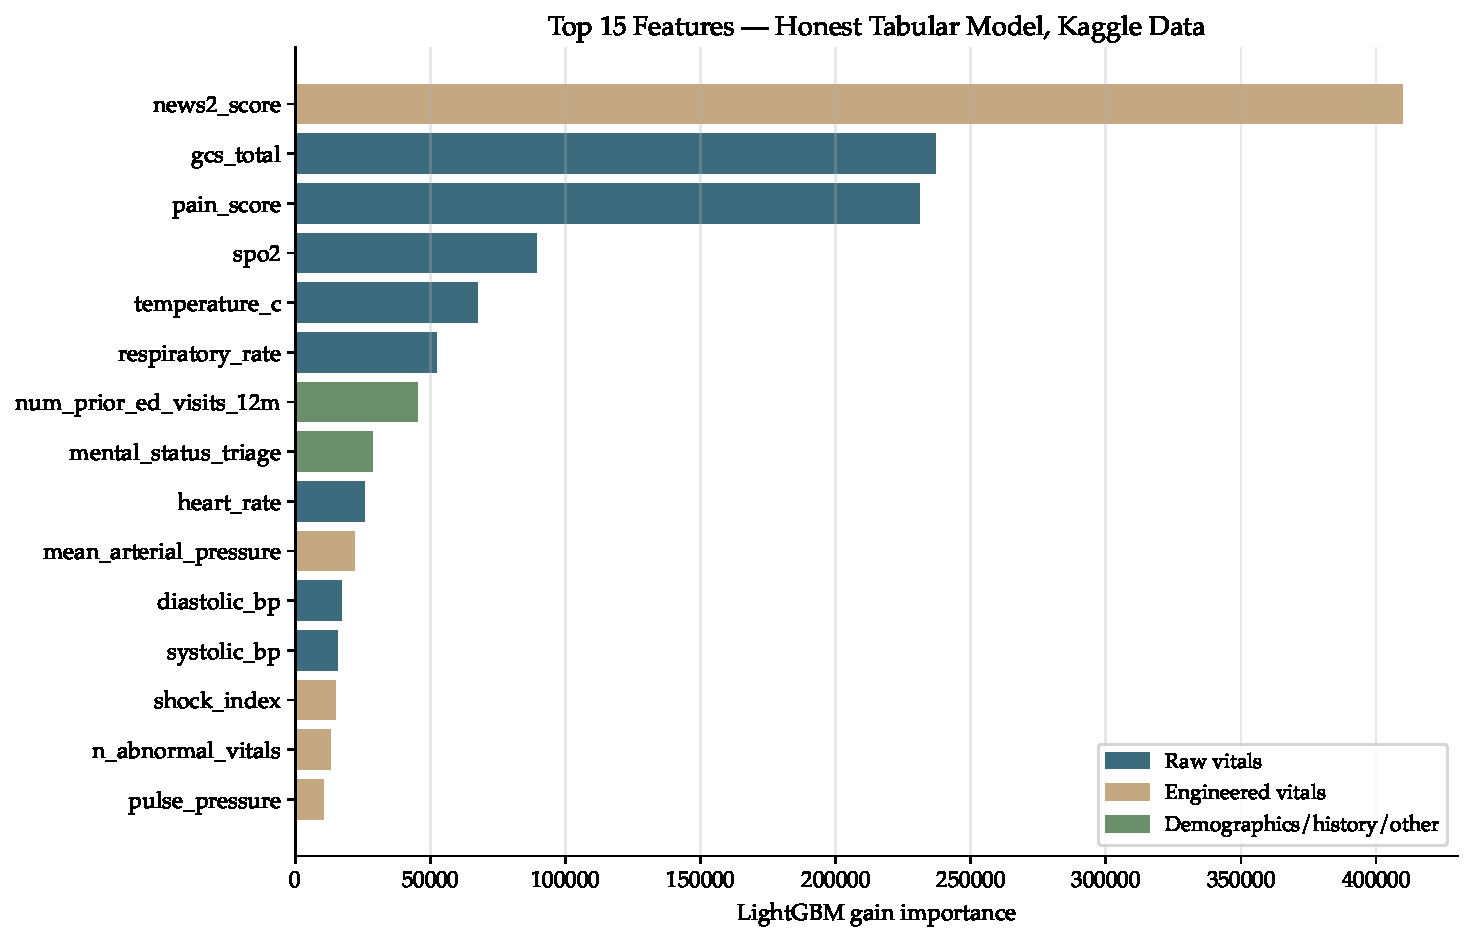
\includegraphics[width=0.95\textwidth]{figures/feature_importance.pdf}
 \caption[Feature importance from the honest tabular baseline]{Gain-importance rankings from the LightGBM baseline on the Kaggle synthetic competition data, trained without text features. The composite clinical scores NEWS2 and GCS dominate, with raw vitals ranked next. This is the ``honest tabular'' model referenced in Chapter~\ref{ch:discovery}, the one that reached F1 $= 0.87$ before text features inflated the score to 0.998. On MIMIC-IV-ED, rankings shift: embedding components become the top features (see Chapter~\ref{ch:embeddings}), but the clinical composite scores remain consistently important. The figure is reproduced here to illustrate the structural role of the engineered features, not the specific numeric values which differ between datasets.}
 \label{fig:feature-importance-kaggle}
\end{figure}
